%bib=bibtex
\documentclass[a4paper,12pt]{article}

\usepackage[utf8]{inputenc}
\usepackage{ifthen,etoolbox}
\usepackage[british]{babel} %languages nicely, with proper date format courtesy of [british]
\usepackage{csquotes} %helps to quotes nicely
%\usepackage{float} %for control over figure positioning

%\usepackage{hyperref} %hyperlinks contents and references
\usepackage{graphicx} %required for image manipulation
\usepackage[a4paper, top=25mm,bottom=25mm,left=25mm,right=25mm]{geometry} %allows manipulation of page structure
\usepackage{cite} %BibTeX bibliography manager
\usepackage{amsmath, amssymb} %adds many fancy maths symbols and things

%\usepackage{epstopdf}
%\usepackage{url}
%\usepackage{setspace}
%\usepackage{titlesec}

\graphicspath{{../../plots/}}

%\usepackage{abstract}
%\addto\captionsenglish{\renewcommand{\abstractname}{}}
%\addto\captionsenglish{\renewcommand{\absnamepos}{empty}}

\title{Analysis Note: Measurement of forward $W$ and $Z$ boson cross sections in $pp$ collisions at $\sqrt{s}=5 \; \rm{TeV}$}
\author{Laura Cairns}
\date{\today}

\begin{document}
\maketitle

\begin{abstract}
    \noindent 
    Measurements of inclusive electroweak boson production cross sections are presented for $pp$ collisions at centre-of-mass energy $\sqrt{s} = 5$ TeV. The data analysed was collected at the LHCb detector with an integrated luminosity of \input{results/lumi_value.tex}. Muon decay channels are studied within the kinematic region defined by pseudorapity $2.0 < \eta < 4.5$ and transverse momenta $p_T > 20$~GeV. The boson cross sections are found to be
    \input{results/Z_xsec_output.tex}
    \input{results/Wp_xsec_output.tex}
    \input{results/Wm_xsec_output.tex}
    where uncertainties are statistical, systematic and due to luminosity respectively. Ratios of these cross sections are also determined as 
    \input{results/WW_ratio_output.tex}
    \input{results/WZ_ratio_output.tex}
\end{abstract}

%%%%%%%%%%%%%%%%%%%%%%%%%%%%%%%%%%%%%%%%%%%%%%%%%%%%%%
\section{Introduction}
The following document presents the results and workflow of an initial analysis of the LHCb 5 TeV dataset, in order to determine the cross sections of electroweak boson production in proton-proton collisions. This was carried out as a Masters project in 2021, with a full report of the findings available.

A number of codes were produced in C++ and \textsc{Python} to do this analysis, which can be run consecutively using the top level script \texttt{run$\_$xsec$\_$analysis.sh}. This document is produce as an output of this analysis. These codes make use of the ROOT framework produced by CERN~\cite{ROOT}. The dataset used is found in the file \texttt{5TeV$\_$2017$\_$32$\_$Down$\_$EW.root}.

%The dataset used in this analysis was collected during Run 2 at the LHCb detector, colliding protons at centre-of-mass energy $\sqrt{s} = 5$ TeV. 
%Before event selection, the dataset contained 5840 $Z$ entries, 373713 $W^+$ entries and 295104 $W^-$ entries.

This document presents the results for the cross sections of the production of $Z, W^+$ and $W^-$ bosons, and the cross section ratios $\sigma_{W^+}/\sigma_{W^-}$ ($R_{W^\pm}$) and $(\sigma_{W^+}+\sigma_{W^-})/\sigma_{Z}$ ($R_{WZ}$). These results are compared to previous LHCb results at different $\sqrt{s}$, and a single theoretical prediction, taken from the supplementary of the 2015 8 TeV LHCb paper~\cite{8TeV_W+Z_2015}, where they were determined using the DYNNLO generator~\cite{DYNNLO} with the MSTW08 parton distribution function~\cite{MSTW08}.
The workflow and results for the determination of luminosity and trigger efficiency are given in Sections~\ref{sec: lumi} and \ref{sec: trig eff} respectively. The workflow and results for the $Z$ boson analysis are given in Section~\ref{sec: Z analysis}. The workflow and results for the $W$ boson analysis and ratio calculation are given in Section~\ref{sec: W analysis}. The comparison to other data is given in Section~\ref{sec: results}.

%%%%%%%%%%%%%%%%%%%%%%%%%%%%%%%%%%%%%%%%

\section{Luminosity} \label{sec: lumi}
The code \texttt{get$\_$luminosity.py} calculates the integrated luminosity $\mathcal{L}$ as the sum of 38 entries, where each entry represents a fraction of the data collected in the 5 TeV run. 
The luminosity in each of these entries was determined prior to this analysis when the LHCb data was processed for offline examination. 
Integrated luminosity and its error are output as a json file ``luminosity.json", for use in subsequent codes.


The error on luminosity is assumed to be 5$\%$.
The full calibration of the integrated luminosity is a complex analysis and has not yet been completed for the 5 TeV run.
Early analyses of the electroweak production at 7 and 13 TeV measured the luminosity to precisions of 3.5$\%$ and 3.9$\%$~\cite{7TeV_W+Z_2012,13TeV_Z_2016}, with the precise analysis of 7 and 8 TeV producing an uncertainty of 1.16$\%$~\cite{LHCb_luminosity}.
Consequently, an estimated uncertainty of 5$\%$ is thought to be a reasonable upper bound on the luminosity precision in this preliminary analysis.

\subsection{Result}
The integrated luminosity $\mathcal{L}$ is found to be:
$\mathcal{L}$ = \input{results/lumi_value.tex}.

%%%%%%%%%%%%%%%%%%%%%%%%%%%%%%%%%%%%%%%%

\section{Trigger Efficiency} \label{sec: trig eff}
The code \texttt{measure$\_$trigger$\_$eff.py} calculates the trigger efficiency $\varepsilon_{\rm trigger}$. The trigger efficiency is determined using the tag-and-probe method, as used in previous LHCb analyses, studing the decay of the $Z$ boson $Z\xrightarrow[]{}\mu^+\mu^-$.
Events where the positive muon or negative muon trigger are counted in the fiducial region (given in Sections~\ref{sec: Z analysis} and \ref{sec: W analysis}), as well as the events where both muons trigger. 
By requiring that one muon triggers (the tag muon) in order for a decay to have occured, then there is no bias on the other muon (the probe muon). Hence, the efficiency of the probe muon trigger may be calculated as the proportion of the successful tag events where both the tag and probe trigger:
\begin{equation}
{\varepsilon}_{{\rm probe \;  muon}} = \frac{{\rm number \; of \; events \; where \; both \; muons \; trigger}}{{\rm number \; of \; events \; where \; tag \; muon \; triggers}}.
\end{equation}

This gives the trigger efficiencies of the positive and negative muons $\varepsilon_{\mu^+}$ and $\varepsilon_{\mu^-}$ as
\begin{equation}
    \varepsilon_{\mu^+} = \frac{N_{\mu^- + \mu^+}}{N_{\mu^-}},
    \label{eq: mup_eff}
\end{equation}
\begin{equation}
    \varepsilon_{\mu^-} = \frac{N_{\mu^- + \mu^+}}{N_{\mu^+}},
    \label{eq: mum_eff}
\end{equation}
where $N$ represents the number of events in the fiducial region where the indicated muon activates a trigger. 
These efficiencies are used in the determination of $W^+$ and $W^-$ cross sections respectively (see Section \ref{sec: W xsec}).
The trigger efficiency used in the $Z$ analysis is calculated as the efficiency of either muon causing a trigger to activate, given as
\begin{equation}
    \varepsilon_{\mu\mu} = \varepsilon_{\mu^+} + \varepsilon_{\mu^-} - \varepsilon_{\mu^+} \times \varepsilon_{\mu^-}.
    \label{eq: either eff}
\end{equation}
The relative uncertainty on each efficiency is determined using the binomial formula $\sqrt{\varepsilon(1-\varepsilon/N}$ where $N$ represents the sample size. In this analysis, $N$ is given as the number of $Z$ events in the fiducial region. The trigger efficiency was assumed to be independent of muon kinematics in this analysis.
The trigger efficiencies and their relative uncertainties are output as a json file ``efficiencies.json", for use in subsequent codes.

\subsection{Results}
Trigger Efficiency = $0.9957 \pm 0.0009$\\Trigger Efficiency Relative Uncertainty = $0.00086$\\


%%%%%%%%%%%%%%%%%%%%%%%%%%%%%%%%%%%%%%%%

\section{$Z$ Boson Analysis} \label{sec: Z analysis}

The code \texttt{measure$\_$xsec.py} calculates the integrated cross section of the Z boson, $\sigma_Z$. The $Z$ signal is assumed to be 100$\%$ pure in this preliminary analysis, with no background subtraction necessary.
Before event selection, the dataset contains 5840 candidate Z events.
Events are selected in the fiducial region, with the number of events $N_{\rm fiducial}$ counted. The fiducial region is comprised of the kinematic cuts:

\begin{itemize}
  \item $60 < M_{\mu\mu} < 120 \; {\rm GeV}$ 
  \item $p_T > 20 \; {\rm GeV}$ for both positive and negative muons
  \item $2.0 < \eta < 4.5$ for both positive and negative muons
\end{itemize}
The statistical uncertainty on $N_{\rm fiducial}$ is given by the Poisson formula $\alpha_N = \sqrt{N}/N$.

$\sigma_Z$ is calculated as
\begin{equation}
\sigma_Z = \frac{N_{\rm fiducial}}{\mathcal{L} \times {\varepsilon_{\rm trigger}}},
\label{eq: Z_xsec}
\end{equation}
using the previously calculated values of integrated luminosity $\mathcal{L}$ and trigger efficiency $\varepsilon_{\rm trigger}$, read in from their respective codes.

Errors are propagated through $\sigma_Z$ according to the equation,
\begin{equation}
    \alpha_\sigma = \sigma \sqrt{\left(\frac{\alpha_N}{N}\right)^2 + \left(\frac{\alpha_\mathcal{L}}{\mathcal{L}}\right)^2 + \left(\frac{\alpha_\varepsilon}{\varepsilon}\right)^2},
    \label{eq: xsec error}
\end{equation}
and given separately in the result as statistical error (from the number of counts), and errors due to efficiency and luminosity. Errors are separated according to the following equation, with the statistical error given as an example;
\begin{equation}
    \alpha_{\sigma {\rm stat}} = \frac{\alpha_N}{N}\sigma.
    \label{eq: xsec error separation}
\end{equation}
%Error analysis on $\sigma_Z$ is carried out using the relative uncertainties on the number of counts, trigger efficiency, and luminosity. Each of these uncertainties is given separately in the result, with the uncertainty on the number of counts representing the statistical error. 
The cross section is output to a json file ``Z$\_$xsec.output" for use in later comparison codes.


\subsection{Results}
Counts in Fiducial Region = $3748 \pm 61 \; \rm counts$\\Counts Relative Uncertainty = $0.0163$\\

\input{results/Z_xsec_output.tex}



%%%%%%%%%%%%%%%%%%%%%%%%%%%%%%%%%%%%%%%%

\section{$W$ Boson Analysis} \label{sec: W analysis}
%%%%%%
\subsection{Comparison of Experimental Data with Monte Carlo Simulation} \label{sec: Z MC comparison}

In the code \texttt{plot$\_$MC$\_$comparison.cpp}, histograms are plotted using ROOT, comparing a number of variables from the 5 TeV LHCb dataset to a Monte Carlo simulation of the experiment. The Monte Carlo simulation was created prior to this analysis using \textsc{Pythia}~\cite{Pythia_6.4,Pythia_8.1}, where $pp$ collisions were generated and passed through detector reconstruction~\cite{LHCb_reconstruction} in order to simulate the expected kinematic distributions of the $Z$ and $W$ decay signals.
This simulation is used to analyse the contributions of the $W$ signal and $Z$ background in the $W$ experimental data, in order to carry out background subtraction and determine the $W$ signal purity.
The $Z$ simulation is compared to the $Z$ experimental data in order to validate the use of these simulations, made possible by the assumption that the $Z$ signal is 100$\%$ pure.
Before event selection, the simulation contains 338926 candidate $Z$ entries.
Simulation data has been scaled to the experimental data in the histogram plots, with each plotted using 80 bins.
The variables compared are:
\begin{itemize}
  \item Transverse Momentum $p_T$, separately for both positive and negative muons
  \item Pseudorapidity $\eta$, separately for both positive and negative muons
  \item Azimuthal angle $\phi$, separately for both positive and negative muons
  \item Dimuon invariant mass $M_{\mu\mu}$, equivalent to the mass of the Z boson $m_Z$.
\end{itemize}

The histograms can be seen in Figure~\ref{fig: Z histograms}.
Differences can be seen between the experimental and simulated data due to background in the experimental data, and inaccuracies in the simulation. These inaccuracies arise due to the leading order precision of \textsc{Pythia} and limits on the precision to which the detector can be described. 

Agreement is seen between the two data sets, validating the use of the $W$ and $Z$ simulations in the $W$ boson background analysis. However, differences can be seen such as the narrow peak of the simulation in the plot of $M_{\mu\mu}$, which suggests that the LHCb reconstruction used in these simulations has estimated a higher detector resolution than exists in experiment. This difference is assumed to be negligible compared to the dominant systematic uncertainty on the $W$ purities, imposed by the $p_T$ event selection in the $K/\pi$ background. More precise analyses of this data should correct for this difference when determining $W$ purity.
Another small difference seen in the plot of $M_{\mu\mu}$ is the small background contamination of the $Z$ data at low $M_{\mu\mu}$. However, this has been removed by the dimuon invariant mass selection criteria on $Z$ candidates, allowing for the assumption of 100$\%$ purity.

\begin{figure*}[p]
\centering
\includegraphics[clip, trim = 0.5cm 0cm 1.7cm 1.2cm, width=0.49\textwidth]{Measurement_1.e-3*mup_PT.pdf}
\includegraphics[clip, trim = 0.5cm 0cm 1.7cm 1.2cm, width=0.49\textwidth]{Measurement_1.e-3*mum_PT.pdf}
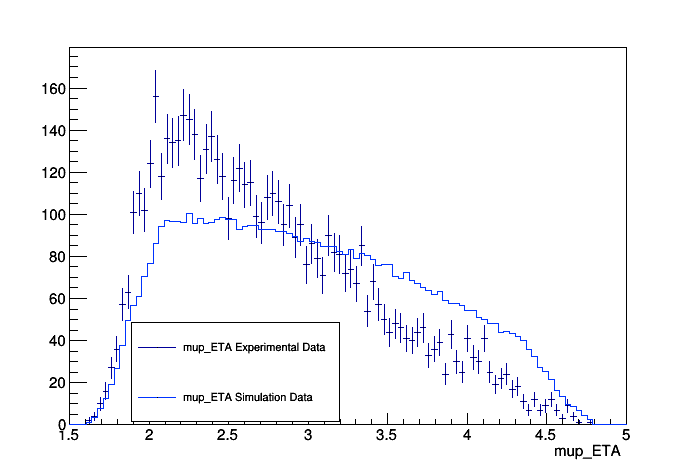
\includegraphics[clip, trim = 0.5cm 0cm 1.7cm 1.2cm, width=0.49\textwidth]{Measurement_mup_ETA.pdf}
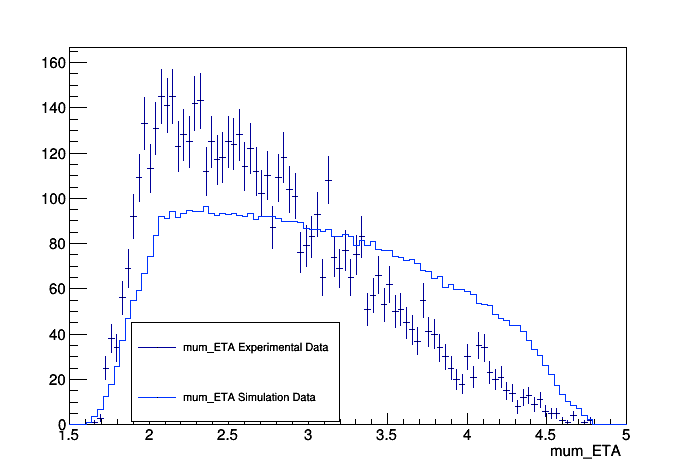
\includegraphics[clip, trim = 0.5cm 0cm 1.7cm 1.2cm, width=0.49\textwidth]{Measurement_mum_ETA.pdf}
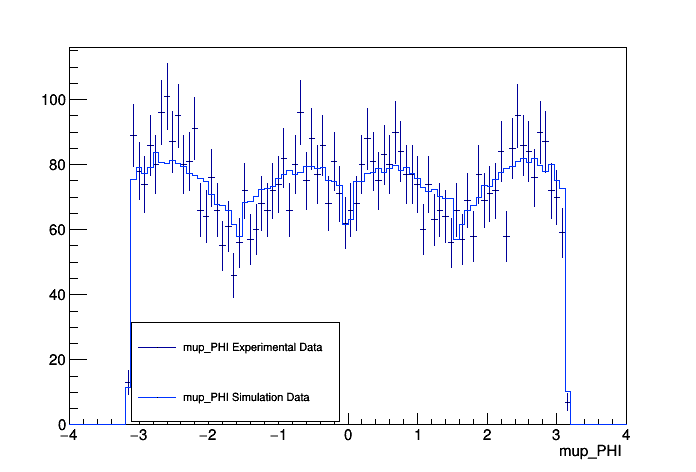
\includegraphics[clip, trim = 0.5cm 0cm 1.7cm 1.2cm, width=0.49\textwidth]{Measurement_mup_PHI.pdf}
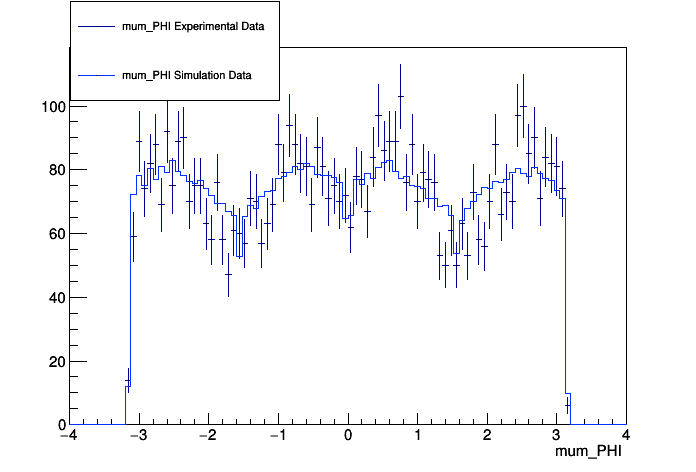
\includegraphics[clip, trim = 0.5cm 0cm 1.7cm 1.2cm, width=0.49\textwidth]{Measurement_mum_PHI.pdf}
\includegraphics[clip, trim = 0.5cm 0cm 1.7cm 1.2cm, width=0.49\textwidth]{Measurement_1.e-3*Z_M.pdf}
\vspace{-4mm}
\caption{\small Comparison of $Z$ experimental data with a Monte Carlo simulation with detector reconstruction. Plots are shown for both positive and negative muons, plotting $M_{\mu\mu}$, $p_T$, $\eta$, and $\phi$.}
\label{fig: Z histograms}
\end{figure*}

%%%%%

\subsection{Plotting W Data} \label{sec: W plotting}

The $p_T$ distributions of $W \xrightarrow{} \mu \nu_\mu$ decays are plotted for both the $W$ experimental data and $W$ signal simulation (discussed in Section~\ref{sec: Z MC comparison}) in the program \texttt{plot$\_$W$\_$dist.cpp}. 
The $W$ signal is isolated by calculating the isolation $p_T^{\rm cone}$; the sum of $p_T$ for all particles surrounding the decay muon in a cone satisfying
\begin{equation}
    \sqrt{\Delta\eta^2 + \Delta\phi^2} < 0.5.
    \label{eq: isolation}
\end{equation}
The inverse of transverse momentum $p_T^{-1}$ are plotted against this isolation, as shown for $W^+$ in Figure \ref{fig: isolation plots}. These figures use the LEGO and COLZ plotting options to highlight different features.
The $W$ decay signal can be seen as a peak between $p_T^{-1}$ = 0.02 and 0.03 GeV$^{-1}$ at low values of isolation, shown prominently in the COLZ plots. The LEGO plots highlight the charged $K/\pi$ background, identified as the Gaussian peak at high $p_T^{-1}$.
Figure~\ref{fig: isolation plots} compares these plots of the experimental data to the simulated $W$ signal data, further highlighting the effects of background in the $W$ experimental data.

\begin{figure*}[t]
\centering
\includegraphics[clip, trim = 0.1cm 0cm 0.3cm 1.3cm, width=0.49\textwidth]{W+_isolated_signal_COLZ_mnt.pdf} %top = 1.3cm
\includegraphics[clip, trim = 0.1cm 0cm 0.3cm 1.3cm, width=0.49\textwidth]{W+_isolated_signal_COLZ_sim.pdf}
\includegraphics[clip, trim = 0.1cm 0.4cm 1.7cm 1.3cm,width=0.49\textwidth]{W+_isolated_signal_mnt.pdf}
\includegraphics[clip, trim = 0.1cm 0.4cm 1.7cm 1.3cm,width=0.49\textwidth]{W+_isolated_signal_sim.pdf}
\vspace{-4mm}
\caption{\small Histogram plots of inverse transverse momentum $p_T^{-1}$ against the log of the isolation $p_T^{\rm cone}$ for the $W^+$ decay. 
Plots of the $W^+$ experimental data (left) and the $W^+$ signal simulation used in background fitting (right) are given, highlighting the effects of background processes on the candidate $W^+$ events.
Both 2D and 3D formats are given to highlight different features; the upper 2D plots highlight the $W^+$ signal between 0.02 and 0.03 GeV$^{-1}$, and the lower 3D plots highlight the hadronic background contamination as a Gaussian peak.}
\label{fig: isolation plots}
\end{figure*}

%%%%%%%%%%%

\subsection{W Background Analysis} \label{sec: W background}

The code \texttt{W$\_$background.cpp} plots and analyses the various background contributions to the $W^+$ and $W^-$ data.

The files used are:
\begin{itemize}
    \item Data: \texttt{5TeV$\_$2017$\_$32$\_$Down$\_$EW.root}
    \item Simulation of W signal: \texttt{5TeV$\_$2015$\_$24r1$\_$Down$\_$W$\_$Sim09d.root}
    \item Simulation of Z production: \texttt{5TeV$\_$2015$\_$24r1$\_$Down$\_$Z$\_$Sim09d.root}
\end{itemize}

The code includes a number of functions which carry out different parts of the analysis, allowing for $W^+$ and $W^-$ data to be analysed simultaneously. The purposes of the functions are as follows:
\begin{itemize}
    \item \texttt{output$\_$histogram}: Plots a histogram from a TH1F object and outputs as a ``png" file, used for testing purposes.
    \item \texttt{make$\_$histogram}: Creates and returns a TH1F histogram from an input decay tree, expression, and cuts.
    \item \texttt{background$\_$fit}: Analyses $K/\pi \xrightarrow{} \mu\nu$ background, fitting the W ``SingleTrackNoBias" trees in the experimental data with an exponential, and returning a Monte Carlo template of the fit. A plot of the exponential fit is output as a ``pdf" file.
    \item \texttt{fraction$\_$fitter}: TFractionFitter is carried out on the background contributions, returning the fractions each comprises in the $W$ data. A plot of this fit is output as a ``pdf" file. 
    \item \texttt{produce$\_$fit$\_$model}: Produces a plot of the fit model, output as a ``pdf" file. Each background contribution is scaled to the data by the fraction calculated in \texttt{fraction$\_$fitter}, and the fit model is calculated as the sum of all background contributions.
    \item \texttt{output$\_$values}: Outputs numerical results of the code to a ``json'' file. The python code \texttt{make$\_$W$\_$latex.py} formats these outputs into latex forms, outputting ``tex'' files, which are input to this document. The output json files are ``Wp$\_$back$\_$output.json" and``Wm$\_$back$\_$output.json".
\end{itemize}
A structure \texttt{fit$\_$fractions} is also introduced to store the fit fractions calculated by the function \texttt{fraction$\_$fitter}. The structure includes the value and error of each fit fraction, along with the string used to label its value in a figure. This forms the output of the function \texttt{fraction$\_$fitter}, and is passed as an input to \texttt{produce$\_$fit$\_$model}.

When creating histogram, the following event selection is carried out, with kinematic cuts carried out on both $W$ and $Z$ histograms, applied to both muons in $Z$.
\begin{itemize}
    \item Kinematic cuts: $p_T >$ 20, 2 $< \eta <$ 4.5
    \item Additional Z cuts: 60 GeV $< M_{\mu\mu} <$ 120 GeV, where $M_{\mu\mu}$ is the invariant mass of the dimuon system; this is equivalent to the mass of the $Z$ boson $m_Z$.
\end{itemize}

The analysis is carried out in the following steps:
\begin{enumerate}
    \item Make and retrieve background templates. Each template is a TH1F histogram of $p_T$ plotted with 50 bins in the range 20 to 60 GeV. This is carried out for both $W^+$ and $W^-$, with the number of events in each histogram after event selection shown in Table \ref{tab: W events}.
    \begin{enumerate}
        \item $K/\pi$ background: Function \texttt{background$\_$fit} is run. $p_T$ is plotted for the Wp and Wm ``SingleTrackNoBias" decay trees in the data file. These decay trees contain high $p_T$ tracks without the requirement for events to be identified as muons (as in the Wp and Wm ``Iso" trees). Hence, these trees contain mostly charged pions $\pi$ and kaons $K$, forming the $K/\pi$ background.
The $p_T$ distribution is plotted with kinematic cuts on eta, a cut on $p_T$ discussed below, and a selection requirement on the track reconstruction of the tree. This requirement forms the cut \texttt{mu$\_$CHI2NDF $<$ 2}, the chi squared per degrees of freedom of the track reconstruction must be less than 2, and removes ghost tracks in the background.
          \newline This distribution is fit with an exponential for three different ranges of $p_T$. This function is run three times for each $W$ boson, with ranges of 15 GeV to 25, 30 and 35 GeV. The 30 GeV fit is used in further analysis to determine the $W$ cross sections, whilst the 25 and 35 GeV fits are used later to determine the systematic uncertainty on the $W$ signal fraction due to uncertainty in the most optimal place to cut at high $p_T$. This cut on $p_T$ helps to ensure that the background template only contains background contributions, removing contamination of the background by $W$ signals at high $p_T$.
The exponential fit is plotted for the 30 GeV fit only, as shown in Figure \ref{fig: W exp back fit}.
          \newline The exponential fit is then used to create the background template. This is a TH1F histogram of 100,000 Monte Carlo events generated from the fit.
          
        \item W Signal: Function \texttt{make$\_$histogram} is run. $p_T$ is plotted for the Wp and Wm ``Iso" decay trees in the W simulation file, with W cuts. These histograms are statistically limited, as seen in Table \ref{tab: W events}.
        
        \item Z background: Function \texttt{make$\_$histogram} is run. $p_T$ is plotted for the Wp and Wm ``Iso" decay trees in the Z simulation file, with W cuts. These histograms are statistically limited, as seen in Table \ref{tab: W events}.
    \end{enumerate}
    
    \item Retrieve $W$ experimental data: The function \texttt{make$\_$histogram} is called. $p_T$ is plotted for the Wp and Wm ``Iso" decay trees in the experimental data, with W cuts in the range 20 to 60 GeV.
    
    \item Calculate Z fraction in W data:
    \begin{enumerate}
        \item Retrieve histograms for $M_{\mu\mu}$ distributions of the ``Z" tree in both data and the $Z$ simulation. The function \texttt{make$\_$histogram} is called for each, using Z cuts.
        \item Calculate the predicted number of $Z$ events in the data of $W^+$ and $W^-$ using
        \begin{equation}
            N_Z[{\rm predicted \; in \;} W {\rm\; data}] = N_W[W {\rm \; in \;} Z {\rm \; simulation}] \times \frac{N_Z[Z {\rm \; data}]}{N_Z[Z {\rm\; simulation}]},
        \end{equation}
        where $N_Z$ is the number of Z events, with the tree counted referred to in square brackets, and $N_W$ is the number of events reconstructed as W in the Z simulation. The fraction of $Z$ in $W$ data, $f_Z$, is then calculated as
        \begin{equation}
            f_Z = \frac{N_Z[{\rm predicted \; in \;} W {\rm\; data}]}{N_W[W {\rm \; data}]}.
        \end{equation}
        [$W$ data] refers to ``WpIso" and ``WmIso" trees, and [$Z$ data] to the ``Z" tree in the data file. \newline
        [$W$ in $Z$ simulation] refers to ``WpIso" and ``WmIso" trees, and [$Z$ simulation] to the ``Z" tree in the $Z$ simulation file. \newline 
        The number of events is counted in each of these trees by taking the integral of their histogram, each retrieved in the above steps. \newline
        The calculated $Z$ fractions are given in Section \ref{sec: W background results}.
        The statistical uncertainty is calculated using the relative uncertainty $\sqrt{N}/N$ on each count in $f_Z$.
        %The number of events in each of these trees is calculated by taking the integral of a histogram of the tree. For the ``W" trees, the $Z$ background and $W$ isolated data histograms discussed above are used, whereas for ``Z" trees, the invariant mass of $Z$ ``Z$\_$M" is plotted with the kinematic cuts used in Section \ref{sec: Z xsec}. 
    \end{enumerate}
    
    \item Run TFractionFitter on the background contributions to determine the fractions they constitute in the $W$ data. The function \texttt{fraction$\_$fitter} is called to do this. The previously determined $Z$ fraction is passed to this function, and is constrained to this value within its statistical uncertainty. This function is called three times for each $W$ boson, using the background templates produced for each $p_T$ range.\newline
    The results of this fit for the 15 GeV $< p_T <$ 30 GeV range are output, producing the plots in Figure \ref{fig: W fraction fit}, and the fit fractions for each background contribution given in Section \ref{sec: W background results}.
    
    \item Calculate the systematic uncertainty on the signal fraction introduced by the shape and fitting of the $K/\pi$ background. This is found by taking the difference between the signal fractions determined with the $p_T$ ranges 15 to 25 GeV and 15 to 35 GeV. This uncertainty is given in Section \ref{sec: W background results}, and in the fit model in Figure~\ref{fig: W fit model}.

    \item Produce the fit model: the function \texttt{produce$\_$fit$\_$model} is called to do this. The $K/\pi$ background template produced using 15 GeV $< p_T <$ 30 GeV range is passed to this function, alongside the templates of $W$ signal and $Z$ background. The histogram of each background contribution is scaled to the $W$ experimental data by
    \begin{equation}
        \frac{{\rm fraction} \times N_W[{\rm W \; data}]}{N[{\rm histogram}]},
    \end{equation}
    where the fraction used is that calculated in the TFractionFitter function.
    The contributions of each background are summed to give the overall fit model, and this is plotted alongside the data and each individual background contribution, as shown in Figure \ref{fig: W fit model}.
\end{enumerate}



%%%%%%%%%%%%
\subsection{Results of Background Analysis} \label{sec: W background results}
% include fit files, events counted in Z fraction calculation,
Results of \texttt{W$\_$background.cpp} are listed below, and include Table~\ref{tab: W events}, and Figures~\ref{fig: W exp back fit}, \ref{fig: W fraction fit}, and \ref{fig: W fit model}.

% Exponential fit of pion kaon background
\begin{figure*}[ht]
  \centering
  \includegraphics[clip, trim = 0.5cm 0.1cm 1.7cm 1.3cm, width=0.49\textwidth]{W+_expo_back_plot.pdf}
  \includegraphics[clip, trim = 0.5cm 0.1cm 1.7cm 1.3cm, width=0.49\textwidth]{W-_expo_back_plot.pdf} \hspace{3mm}
  \vspace{-4mm}
  \caption{\small Exponential Fits of $p_T$ distributions for $W^+$ (left) and $W^-$ (right) in the ``SingleTrackNoIso" trees; high $p_T$ tracks without a muon identification requirement.
  The fit parameters of the function ${\rm p}_0e^{-{\rm p}_1x}$ are given, alongside the $\chi^2/{\rm ndf}$ of the fit. Mostly comprised of charged pions and kaons, this forms the template of the $K/\pi$ background.} 
  
  % Top plots show these tracks plotted with a requirement on the chi squared per ndf to be less than 2. The bottom plots do not include this cut.
  \label{fig: W exp back fit}
\end{figure*}

% Table of event numbers
\input{results/W_event_table_output.tex}

% Z fractions
\textbf{The $Z$ fractions are calculated to be}: \newline
\input{results/Wp_Z_frac_output.tex}
\input{results/Wm_Z_frac_output.tex}

% Fit fractions
\textbf{The background fractions are determined by TFractionFitter to be:} \newline
\input{results/Wp_fit_fracs_output.tex}
\newline
\input{results/Wm_fit_fracs_output.tex}

% Fraction fitter plots
\begin{figure*}[hbt]
\centering
\includegraphics[clip, trim = 0.1cm 0cm 1.7cm 1.2cm, width=0.49\textwidth]{W+_fraction_fit.pdf}
\includegraphics[clip, trim = 0.1cm 0cm 1.7cm 1.2cm, width=0.49\textwidth]{W-_fraction_fit.pdf} 
\vspace{-4mm}
\caption{\small Plots of fits produced by TFractionFitter carried out on $W^+$ (left) and $W^-$ (right) data, with background fractions from $K/\pi \xrightarrow{} \mu\nu$, $W$ signal, and $Z \xrightarrow{} \mu\mu$. Crosses indicate the $W$ data, and the line indicates the fit. The $\chi^2/$degrees of freedom of the fit is given.} %The top plots include a requirement on the track reconstruction examined in the background template, which is not included in the bottom plots.
\label{fig: W fraction fit}
\end{figure*}

% Fit model plots
\begin{figure*}[ht]
\centering
\includegraphics[clip, trim = 0.1cm 0cm 1.7cm 1.2cm, width=0.49\textwidth]{W+_fit_model.pdf}
\includegraphics[clip, trim = 0.1cm 0cm 1.7cm 1.2cm, width=0.49\textwidth]{W-_fit_model.pdf} 
\vspace{-4mm}
\caption{\small Background fitting of $W^+$ (left) and $W^+$ (right). The experimental data are indicated as points with error bars, and the fit model is plotted in black, calculated as the sum of the $W$ signal and all background contributions. Separate contributions are plotted for the hadronic $K/\pi$ background (blue), the $W \xrightarrow{} \mu \nu_\mu$ decay signal (red), and the $Z \xrightarrow{} \mu\mu$ decay background (green). 
The fractions of the fit model formed by each contribution are given with their statistical uncertainty, alongside the systematic uncertainty on the $W$ signal introduced by the $K/\pi$ background event selection, and the $\chi^2/$ndf of the fraction fitting to the experimental data.}
\label{fig: W fit model}
\end{figure*}


\subsection{$W$ Cross Section and Cross Section Ratio Determination} \label{sec: W xsec}
The code \texttt{measure$\_$W$\_$xsec.py} calculates the $W^+$ and $W^-$ cross sections, and calculates the cross section ratios $\sigma_{W^+}/\sigma_{W^-}$ ($R_{W^\pm}$) and $\sigma_{W}/\sigma_{Z}$ ($R_{WZ}$). Values used in this calculation are read in from json files produced in the codes \texttt{W$\_$background.cpp}, \texttt{get$\_$luminosity.py}, and \texttt{measure$\_$trigger$\_$eff.py}, (see Sections \ref{sec: W background}, \ref{sec: lumi}, and \ref{sec: trig eff} respectively). The $Z$ cross section results are calculated in this code using the same method as discussed in Section~\ref{sec: Z analysis} rather than read in again from the json file produced by the $Z$ xsec code; this avoids floating point errors in the calculation of the ratios.
Results are output as json files, ``Wp$\_$xsec.json", ``Wm$\_$xsec.json", and ``Ratios.json". These are formatted to tex files in the code \texttt{make$\_$W$\_$latex.py}, similarly to \texttt{W$\_$background.cpp}.
The results of this analysis are given in Section~\ref{sec: results}.

\subsubsection{$W$ Cross Sections} 
Each cross section is determined in the function \texttt{xsec$\_$calc}. Background subtraction is carried on the $W$ experimental data, determining the expected number of $W$ events in the signal $N_{\rm signal}$ as
\begin{equation}
    N_{\rm signal} = N_W \times \rho_{\rm signal},
    \label{eq: signal frac}
\end{equation}
where $N_W$ is the total number of $W$ events in the data after event selection, and $\rho_{\rm signal}$ is the signal fraction determined in the background fitting, both found in \texttt{W$\_$background.cpp} (Section \ref{sec: W background}). 
$N_{\rm signal}$ contains both statistical uncertainties due to the number of events and the background fitting, and systematic uncertainty due to the $K/\pi$ background event selection.
The statistical error on $N_{\rm signal}$ forms the statistical error on the cross section measurement, and is determined as
\begin{equation}
    \frac{\alpha_{N_{\rm signal \; stat}}}{N_{\rm signal}} = \sqrt{\left(\frac{\alpha_{\rho_{\rm signal \; stat}}}{\rho_{\rm signal}}\right)^2 + \left(\frac{\sqrt{N_W}}{N_W}\right)^2} .
\end{equation}
The cross section of each $W$ boson $\sigma_W$ is subsequently calculated as
\begin{equation}
    \sigma_W = \frac{N_{\rm signal}}{\mathcal{L} \times \varepsilon_{\rm trigger}},
    \label{eq: W_xsec}
\end{equation}
where $\mathcal{L}$ is luminosity and $\varepsilon_{\rm trigger}$ is the trigger efficiency. The error on this value is given separately as statistical error, systematic error (due to trigger efficiency and $K/\pi$ background fitting), and luminosity error, determined using Equations~\ref{eq: xsec error} and \ref{eq: xsec error separation}.
The trigger efficiencies used here are $\varepsilon_{\mu^+}$ and $\varepsilon_{\mu^-}$ for $W^+$ and $W^-$ respectively, as given in Equations~\ref{eq: mup_eff} and \ref{eq: mum_eff}. These are calculated in the program \texttt{measure$\_$trigger$\_$eff.py} and their values given in Section~\ref{sec: trig eff}. 

As $W$ boson decays only produce one muon, there is no redundancy with which to calculate trigger efficiency; if a muon does not activate a trigger, no event will be counted. The muon will either trigger or not. Conversely, in the $Z$ boson decay, two muons are produced, allowing for the trigger efficiency to be measured according to whether one or both muons activate the trigger in each event. Hence, the trigger efficiency has to be calculated using the $Z$ boson data rather than $W$. It is assumed that the trigger efficiency is independent of the muon kinematics.

The $W$ cross sections are found to be
\input{results/Wp_xsec_output.tex}
\input{results/Wm_xsec_output.tex}

% WW Ratio
\subsubsection{$W^\pm$ Ratio}
The ratio of  $W^+$ to $W^-$ boson cross sections $\sigma_{W^+}/\sigma_{W^-}$, $R_{W^\pm}$, is calculated as follows, given in terms of Equations~\ref{eq: W_xsec} for purposes of error propagation,
\begin{equation}
    R_{W^\pm} = \frac{\sigma_{W^+}}{\sigma_{W^-}} = \frac{N_{W^+}}{\varepsilon_{\mu^+}} \cdot \frac{\varepsilon_{\mu^-}}{N_{W^-}},    
\end{equation}
where $N_{W^+}$ and $N_{W^-}$ are the $N_{\rm signal}$ used in $\sigma_{W^+}$ and $\sigma_{W^-}$ determination respectively.
As luminosity cancels from this equation, the large errors imposed on the cross section measurements by luminosity can be ignored.
This leaves the statistical and systematic errors as the only error contributions.
Hence, errors can be propagated as,
\begin{equation}
    \alpha_{W^\pm} = R_{W^\pm}\sqrt{\left(\frac{\alpha_{N_{W^+}}}{N_{W^+}}\right)^2 + \left(\frac{\alpha_{N_{W^-}}}{N_{W^-}}\right)^2 + \left(\frac{\alpha_{\varepsilon_{\mu^+}}}{\varepsilon_{\mu^+}}\right)^2 + \left(\frac{\alpha_{\varepsilon_{\mu^-}}}{\varepsilon_{\mu^-}}\right)^2}.
\end{equation}
Using Equation~\ref{eq: xsec error separation}, this can be set in terms of the statistical and systematic errors of $\sigma_{W^+}$ and $\sigma_{W^-}$ as,
\begin{equation}
       \alpha_{W^\pm} = R_{W^\pm}\sqrt{\left(\frac{\alpha_{\sigma_{W+} \rm stat}}{\sigma_{W+}}\right)^2 + \left(\frac{\alpha_{\sigma_{W-}\rm stat}}{\sigma_{W-}}\right)^2 + \left(\frac{\alpha_{\sigma_{W+} \rm sys}}{\sigma_{W+}}\right)^2 + \left(\frac{\alpha_{\sigma_{W-}\rm sys}}{\sigma_{W-}}\right)^2},
       \label{eq: WW errors}
\end{equation}
\begin{equation}
    {\rm where \;} \left(\frac{\alpha_{\sigma_{W}\rm stat}}{\sigma_{W}}\right)^2 = \left(\frac{\alpha_{N_{W \rm stat}}}{N_{W}}\right)^2 {\rm \; and \;} \left(\frac{\alpha_{\sigma_{W} \rm sys}}{\sigma_{W}}\right)^2 = \left(\frac{\alpha_{N_{W \rm sys}}}{N_{W}}\right)^2 + \left(\frac{\alpha_{\varepsilon_{\mu}}}{\varepsilon_{\mu}}\right)^2.
\end{equation}
The statistical and systematic errors on the cross sections in Equation~\ref{eq: WW errors} are grouped together to find the statistical and systematic errors on $R_{W^\pm}$, giving the final separated errors as follows, with the statistical error given as an example:
\begin{equation}
    \alpha_{W^\pm \rm stat} = R_{W^\pm}\sqrt{\left(\frac{\alpha_{\sigma_{W+} \rm stat}}{\sigma_{W+}}\right)^2 + \left(\frac{\alpha_{\sigma_{W-}\rm stat}}{\sigma_{W-}}\right)^2}.
\end{equation}
The $\sigma_{W^+}/\sigma_{W^-}$ ratio is found to be
\input{results/WW_ratio_output}

\subsubsection{WZ Ratio}
% WZ Ratio
The ratio of $W$ to $Z$ boson cross sections $\sigma_{W}/\sigma_{Z}$, $R_{WZ}$, is calculated using cross sections, with the ratio given in terms of Equation~\ref{eq: W_xsec} for purposes of error propagation:
\begin{equation}
    R_{WZ} = \frac{\sigma_{W^+} + \sigma_{W^-}}{\sigma_{Z}} = \left( \frac{N_{W^+}}{\varepsilon_{\mu^+}} + \frac{N_{W^-}}{\varepsilon_{\mu^-}} \right) \cdot \frac{\varepsilon_{\mu\mu}}{N_{Z}},
\end{equation}
where $\varepsilon_{\mu\mu}$ is the trigger efficiency of either muon in a $Z$ decay, given in Equation~\ref{eq: either eff}, and $N_Z$ is $N_{\rm fiducial}$ in Equation~\ref{eq: Z_xsec}.
Similarly to $R_{W^\pm}$, luminosity cancels, removing it from error propagation. The error on $R_{WZ}$ can be propagated as follows, with coefficients $A$ and $B$ given below,
\begin{equation}
        \frac{\alpha_{WZ}}{R_{WZ}} = \sqrt{
            A\cdot\left(\frac{\alpha_{N_{W^+}}}{N_{W^+}}\right)^2 + B\cdot\left(\frac{\alpha_{N_{W^-}}}{N_{W^-}}\right)^2 + \left(\frac{\alpha_{N_{Z}}}{N_{Z}}\right)^2 + A\cdot\left(\frac{\alpha_{\varepsilon_{\mu^+}}}{\varepsilon_{\mu^+}}\right)^2 + B\cdot\left(\frac{\alpha_{\varepsilon_{\mu^-}}}{\varepsilon_{\mu^-}}\right)^2 + \left(\frac{\alpha_{\varepsilon_{\mu\mu}}}{\varepsilon_{\mu\mu}}\right)^2
        },
\end{equation}
\begin{equation}
    A = \left(\frac{N_{W^+}}{\varepsilon_{\mu^+}}\right)^2 \bigg/ \left(\frac{N_{W^+}}{\varepsilon_{\mu^+}} + \frac{N_{W^-}}{\varepsilon_{\mu^-}}\right)^2, \quad {\rm and} \quad B = \left(\frac{N_{W^-}}{\varepsilon_{\mu^-}}\right)^2 \bigg/ \left(\frac{N_{W^+}}{\varepsilon_{\mu^+}} + \frac{N_{W^-}}{\varepsilon_{\mu^-}}\right)^2.
\end{equation}
Using Equation~\ref{eq: xsec error separation}, this can be set in terms of the statistical and systematic errors of $\sigma_{W^+}$ and $\sigma_{W^-}$ as,
\begin{equation}
        \alpha_{WZ} = R_{WZ}\sqrt{
            \begin{aligned}
                A \cdot \left(\frac{\alpha_{\sigma_{W+} \rm stat}}{\sigma_{W+}}\right)^2 + B \cdot \left(\frac{\alpha_{\sigma_{W-}\rm stat}}{\sigma_{W-}}\right)^2 + \left(\frac{\alpha_{\sigma_{Z}\rm stat}}{\sigma_Z}\right)^2 \\
                + A \cdot \left(\frac{\alpha_{\sigma_{W+} \rm sys}}{\sigma_{W+}}\right)^2 + B \cdot \left(\frac{\alpha_{\sigma_{W-}\rm sys}}{\sigma_{W-}}\right)^2 + \left(\frac{\alpha_{\sigma_{Z}\rm eff}}{\sigma_Z}\right)^2 \\
            \end{aligned}
        },
        \label{eq: WZ errors}
\end{equation}
\begin{equation}
    {\rm where \;} \left(\frac{\alpha_{\sigma_{W}\rm stat}}{\sigma_{W}}\right)^2 = \left(\frac{\alpha_{N_{W \rm stat}}}{N_{W}}\right)^2 {\rm \; and \;} \left(\frac{\alpha_{\sigma_{W} \rm sys}}{\sigma_{W}}\right)^2 = \left(\frac{\alpha_{N_{W \rm sys}}}{N_{W}}\right)^2 + \left(\frac{\alpha_{\varepsilon_{\mu}}}{\varepsilon_{\mu}}\right)^2.
\end{equation}
The statistical and systematic errors on the cross sections are grouped together to find the statistical and systematic errors on $R_{WZ}$, as before for $R_{W^\pm}$, with statistical error given as an example:
\begin{equation}
    \alpha_{WZ \rm stat} = R_{WZ}\sqrt{A \cdot \left(\frac{\alpha_{\sigma_{W+} \rm stat}}{\sigma_{W+}}\right)^2 + B \cdot \left(\frac{\alpha_{\sigma_{W-}\rm stat}}{\sigma_{W-}}\right)^2 + \left(\frac{\alpha_{\sigma_{Z}\rm stat}}{\sigma_Z}\right)^2}
\end{equation}
The $\sigma_{W}/\sigma_{Z}$ ratio is found to be
\input{results/WZ_ratio_output}


%\subsection{Results of W Analysis}
%The results of this analysis are as follows:
%\input{results/Wp_xsec_output.tex}
%\input{results/Wm_xsec_output.tex}
%\input{results/WW_ratio_output.tex}
%\input{results/WZ_ratio_output.tex}

\section{Main Results and Comparison} \label{sec: results}
The overall results of the entire analysis are as follows; electroweak production in $pp$ collisions at $\sqrt{s}=5$ TeV,
\input{results/Z_xsec_output.tex}
\input{results/Wp_xsec_output.tex}
\input{results/Wm_xsec_output.tex}
\input{results/WW_ratio_output.tex}
\input{results/WZ_ratio_output.tex}

Breakdowns of the statistical and systematic errors due to each source are given for each result in Tables~\ref{tab: statistical uncertainties} and \ref{tab: systematic uncertainties}.

\input{results/stat_unc_table_output.tex}
\input{results/sys_unc_table_output.tex}

The cross sections are compared to published LHCb data in Figures~\ref{fig: xsec comparison} and \ref{fig: all xsec comparison}. The cross section are determined for the same fiducial region in for each centre of mass energy $\sqrt{s}$, with $W$ boson cross sections are compared to values determined at 7 and 8 TeV~\cite{7TeV_Z_2015,8TeV_W+Z_2015}, and to values at 7, 8 and 13 TeV for the $Z$ boson cross section~\cite{7TeV_Z_2015,8TeV_W+Z_2015,13TeV_Z_2016}.
The cross section ratios are compared at 7 and 8 TeV in Figure~\ref{fig: ratio comparison}, using the same LHCb publications as the $Z$ boson cross sections~\cite{7TeV_Z_2015,8TeV_W+Z_2015}.
These comparison figures are plotted in the codes \texttt{plot$\_$xsec.py} and \texttt{plot$\_$all$\_$xsecs.py}. 
Additionally, theoretical values of the each boson cross section and the cross section ratios are included in the comparison figures, shown as red trends. These values have been taken from the supplementary of the 2015 8 TeV LHCb paper~\cite{8TeV_W+Z_2015}, where they were determined using the DYNNLO generator~\cite{DYNNLO} with the MSTW08 parton distribution function~\cite{MSTW08}.
In order to highlight the dominant effect of the systematic uncertainties on the 5 TeV cross sections and ratios measured in this analysis, separate error bars for the statistical and total uncertainties are plotted. 

It is observed in Figure~\ref{fig: all xsec comparison} that the 5 TeV cross section for each boson is shifted above their theoretical value by roughly the same amount. This is determined to be a factor around 1.6, with the specific factor differences between experimental and theoretical 5 TeV cross sections given below. As this difference is present in all three boson cross sections, and the ratios are in agreement with theory, it is suggested that this difference arise due to the luminosity.

\input{results/theory_exp_factor_difference.tex}

The code \texttt{plot$\_$W$\_$xsec.py} is additionally available to produce a zoomed in comparison plot of the two $W$ boson cross sections to published data and theory. The plot produced by this code was used in the final report produced for this analysis as part of the Masters project.

%\begin{table}[ht]
%    \centering
%    \begin{tabular}{c|ll}
%        \hline
%         Energy (TeV)   & $R_{W^\pm}$ & $R_{WZ}$  \\
%        \hline
%         5              & \input{results/WW_value.tex}  & \input{results/WZ_value.tex}  \\
%         7              & 1.274 $\pm$ 0.005 $\pm$ 0.009 $\pm$ 0.002 & 20.63 $\pm$ 0.09 $\pm$ 0.12 $\pm$ 0.05  \\
%         8              & 1.336 $\pm$ 0.004 $\pm$ 0.005 $\pm$ 0.002 & 20.13 $\pm$ 0.06 $\pm$ 0.11 $\pm$ 0.4   \\
%         \hline
%   \end{tabular}
%    \caption{\small Comparison of cross section ratios determined at LHCb at $\sqrt{s} =$ 5, 7, and 8 TeV. Errors are statistical, systematic, and due to beam energy respectively~\cite{7TeV_Z_2015,8TeV_W+Z_2015}.}
%    \label{tab: ratio comparison}
%\end{table}

%There is good agreement between our $R_{W^\pm}$ ratio and published results. However, our $R_{WZ}$ ratio is higher than these previous results. This would suggest that either the determined $Z$ cross section is too small, or the $W$ cross sections could be too large. Comparing the $W$ cross sections at each energy (as seen in Table~\ref{tab: xsec comparison}), I would propose that the $W$ cross sections are too large; there is a significant difference between 7 and 8 TeV, which is not seen between 5 and 7 TeV. For this larger gap in energy, I would expect a large difference in cross section, as seen in the $Z$ cross section. These differences will become more apparent in plotting the cross sections as a function $\sqrt{s}$, the next step in this analysis.

%\begin{table}[ht]
%    \centering
%    \footnotesize
%    \begin{tabular}{c|lll}
%        \hline
%         $\sqrt{s}$ (TeV)   &  $\sigma_{Z}$ (pb) &  $\sigma_{W^+}$ (pb) &  $\sigma_{W^-}$ (pb)  \\
%        \hline
%         5              &  \input{results/Z_xsec_value.tex}  &  \input{results/Wp_xsec_value.tex} &  \input{results/Wm_xsec_value}\\
%         7              &  76.0 $\pm$ 0.3 $\pm$ 0.5 $\pm$ 1.0 $\pm$ 1.3 &  878.0 $\pm$ 2.1 $\pm$ 6.7 $\pm$ 9.3 $\pm$ 15.0 &  689.5 $\pm$ 2.0 $\pm$ 5.3 $\pm$ 6.3 $\pm$ 11.8\\
%         8              &  95.0 $\pm$ 0.3 $\pm$ 0.7 $\pm$ 1.1 $\pm$ 1.1 &  1093.6 $\pm$ 2.1 $\pm$ 7.2 $\pm$ 10.9 $\pm$ 12.7 &  818.4 $\pm$ 1.9 $\pm$ 5.0 $\pm$ 7.0 $\pm$ 9.5\\
%         \hline
%    \end{tabular}
%    \caption{\small Comparison of cross sections determined at LHCb at $\sqrt{s} =$ 5, 7, and 8 TeV. Errors on 5 TeV values are statistical, systematic, and luminosity. On 7 and 8 TeV values, the errors are statistical, systematic, due to beam energy, and luminosity. The 7 TeV values were measured at luminosity of 1.0 fb$^{-1}$, and 8 TeV values at 2.0 fb$^{-1}$~\cite{7TeV_Z_2015,8TeV_W+Z_2015}.}
%    \label{tab: xsec comparison}
%\end{table}

\begin{figure*}[t]
\centering
\includegraphics[clip, trim = 0.2cm 0.2cm 1.9cm 1.3cm, width = 0.49\textwidth]{Wp_xsec_plot.pdf}
\includegraphics[clip, trim = 0.2cm 0.2cm 1.9cm 1.3cm, width = 0.49\textwidth]{Wm_xsec_plot.pdf}
\includegraphics[clip, trim = 0.2cm 0.2cm 1.9cm 1.3cm, width = 0.49\textwidth]{Z_xsec_plot.pdf}
\vspace{-4mm}
\caption{\small Comparisons of measured fiducial cross sections (green) with published LHCb results (black) at 7, 8 and 13 TeV~\cite{7TeV_Z_2015,8TeV_W+Z_2015,13TeV_Z_2016}. 
Error bars for both the total uncertainty (outer) and the statistical uncertainty (inner) are plotted for the 5 TeV data, with the statistical error too small to see for $Z$. Error bars are too small to be seen on the 7 and 8 TeV $Z$ data.
The theoretical relationship between cross section and centre of mass energy $\sqrt{s}$ is also included (red), which have been taken from the supplementary of the 2015 8 TeV LHCb paper~\cite{8TeV_W+Z_2015}, where they were determined using the DYNNLO generator~\cite{DYNNLO} with the MSTW08 parton distribution function~\cite{MSTW08}.}
\label{fig: xsec comparison}
\end{figure*}

\begin{figure}[ht]
\centering
\includegraphics[clip, trim = 0.5cm 0.2cm 1.9cm 1.3cm, width = 0.65\textwidth]{all_xsecs_plot.pdf}
\vspace{-3mm}
\caption{\small Comparisons of the fiducial cross sections $\sigma$ of $W^+$, $W^-$, and $Z$ bosons measured in this report (green) with published LHCb results (black) at 7, 8 and 13 TeV~\cite{7TeV_Z_2015,8TeV_W+Z_2015,13TeV_Z_2016}. 
Error bars for both the total uncertainty (outer) and the statistical uncertainty (inner) are plotted for the 5 TeV data, with the statistical error too small to see for $Z$. Error bars are too small to be seen on the 7 and 8 TeV $Z$ data.
The theoretical relationship between cross section and centre of mass energy $\sqrt{s}$ is also included (red), which have been taken from the supplementary of the 2015 8 TeV LHCb paper~\cite{8TeV_W+Z_2015}, where they were determined using the DYNNLO generator~\cite{DYNNLO} with the MSTW08 parton distribution function~\cite{MSTW08}.}
\label{fig: all xsec comparison}
\end{figure}

\begin{figure*}[t]
\centering
\includegraphics[clip, trim = 0.3cm 0.2cm 1.9cm 1.3cm, width = 0.49\textwidth]{WW_ratio_plot.pdf}
\includegraphics[clip, trim = 0.3cm 0.2cm 1.9cm 1.3cm, width = 0.49\textwidth]{WZ_ratio_plot.pdf} % optimum left cut is 0.7cm, but set to 0.3cm for consistency
\vspace{-4mm}
\caption{\small Comparisons of the fiducial cross section ratios calculated in this analysis (green) with published LHCb results (black) at 7 and 8 TeV~\cite{7TeV_Z_2015,8TeV_W+Z_2015}. 
Error bars for both the total uncertainty (outer) and the statistical uncertainty (inner) are plotted for the 5 TeV data, with error bars too small to see for 7 and 8 TeV.
The theoretical relationship between the ratios and centre of mass energy $\sqrt{s}$ is also included (red), which have been taken from the supplementary of the 2015 8 TeV LHCb paper~\cite{8TeV_W+Z_2015}, where they were determined using the DYNNLO generator~\cite{DYNNLO} with the MSTW08 parton distribution function~\cite{MSTW08}.} 
\label{fig: ratio comparison}
\end{figure*}


%\section{Future Work} \label{sec: future work}
%\subsection{Monte Carlo Comparison of Z data for 5 TeV Measurement} \label{Z histograms}
%The use of the simulations used in data analysis should be validated by comparison with the $Z$ experimental data. 
%The plots in Figure~\ref{fig: Z histograms} are comparisons of the $Z$ data with a Monte Carlo simulation of $Z$ produced at $\sqrt{s}=$5 TeV which had undergone detector reconstruction (\texttt{5TeV$\_$2015$\_$24r1$\_$Down$\_$Z$\_$Sim09d.root}). 
%%%%% The plots in Figure~\ref{fig: Z histograms} are comparisons of the $Z$ data with a Monte Carlo simulation of $Z$ produced at $\sqrt{s}=$13 TeV which had undergone detector reconstruction (\texttt{13TeV$\_$2016$\_$28r1$\_$Down$\_$Z$\_$Sim09h.root}). 
%The simulation data has been scaled to the experimental data, each histogram plotted with 100 bins. 

%Comparison of these plots can be used to correct for imperfections in the detector and to remove background from measurements, although the simulation is limited in precision to leading order by \textsc{Pythia} and by the precision to which the detector can be described.




\bibliography{measurement_report}
\bibliographystyle{h-physrev5}

\end{document}
